%!TEX root = ../thesis.tex

\chapter{Separating the spectra of faint companions} % Main chapter title
\label{cha:direct_recovery}

This chapter focuses on applying a direct subtraction method to near-infrared (\nir{}) spectra of {FGK} stars which have Brown Dwarf (BD) companions, with the goal to isolate the spectrum of the companions and determine their mass from the radial velocity difference.
The data used was obtained with the {CRIRES} instrument in 2012\footnote{Before this thesis began} observed with the purpose to apply the differential technique specifically.
A level of trust was placed in the quality of the observations, which was unfortunately misplaced.
This chapter begins by presenting a range of spectral separation techniques, followed by the motivation for the specific targets observed and details about the observations obtained.
The direct subtraction technique is presented and its application to the observations is explored.
The limits of the differential technique at low {RV} separations is given by simulation with synthetic spectra.

%!TEX root = ../../thesis.tex

\section{Spectral separation techniques}
\label{sec:disentangling_techniques}

Spectral observations of binary systems contain the spectra of both bodies, in proportion to their flux ratio, and are Doppler shifted relative to each other due to their orbital motion.
There are many disentangling techniques to separate mixed spectra of binary systems,~\citep[e.g.][and references therein]{hadrava_disentangling_2009}.
These techniques were initially developed to identify and separate the spectra of binary stars, however the techniques and instrumentation have improved so that lower flux ratios from smaller BD and giant planet companions have begun to be detected.
A small variety of these techniques will be briefly presented below before exploring the techniques used in this work in more depth.

Several disentangling techniques work on deriving the spectral components from several spectra at different orbital phases.
At the minimum \(n+1\) observations can be used to set up a system of linear equations to solve for \(n\) spectral components.
Each observation adds independent information to the system, with no redundant information, that is it cannot be reduced to a system of few equations with the same information.
Works such as \citet[][]{simon_disentangling_1994, sablowski_spectral_2016} use singular value decomposition {SVD} to solve the system for the spectral components.
These work best with many well spaced observations, for example~\citet{sablowski_spectral_2016} state their ideal situation is homogeneous samples over at least half the period, to identify the moving spectral components.
Each extra spectrum in the system adds unique information, with no redundant  

Tomographic techniques~\citep[e.g.][]{bagnuolo_tomographic_1991} and Fourier techniques~\citep{hadrava_orbital_1995} have also been developed for disentangling a series of binary spectra.
Recently this has even been performed using Gaussian processes which simultaneously fits stellar (or exoplanet) orbits as well as their spectral components~\citep{czekala_disentangling_2017}.

A fairly common technique for deriving precise radial velocities of spectral components in binaries is to apply cross-correlation against a library of known spectra.
{TODCOR} (TwO-Dimensional CORrelation)~\citep{zucker_study_1994} is a commonly used algorithm for cross-correlation of two spectral components to revealing the {RV} of both components.
It has been simulated to be able to detect secondaries with flux ratios down to \(\sim\)1/1000 provided a sufficient \snr{}~\citep[e.g.][]{mazeh_todcor_1994,mazeh_detecting_1997}.
{TODCOR} requires knowledge of the two spectral components; a series of spectral templates are used to correlate against the observation.
These can either be other observed or synthetic stellar spectra, with the highest correlating spectral pair indicating the two components.

Recently this has been used to detect the emission spectra of non-transiting giant planets.
\citet{lockwood_nearir_2014} and~\citet{piskorz_evidence_2016} apply TODCOR, with specialized exoplanet spectrum templates used for the companion, to several epochs of high resolution and high \snr{} \nir{} spectra.
They combine together the individual results in a maximum likelihood framework to obtain the orbital solution of the components.

\textchisquared{} fitting of observations to a library of spectra can also be performed.
\citet{kolbl_detection_2015} perform spectral fitting against the {SpecMatch} library of observed optical spectra, achieving an 80\% injection-recovery rate for a 3500\K{} {M-dwarf} companion to an 5000--6000\K{} host star at a 1\% flux ratio.
Unfortunately a thorough high-resolution spectral library in the \nir{} is not currently available, requiring synthetic spectral libraries to be used in this work instead.

Other methods for spectral separation focus on removing the spectral component of the host star.
\citet{rodler_weighing_2012} do this by constructing a stellar mask for the host by constructively combining the host spectra from a number of different phases.
The contribution of the faint companion to the mask, added at different phases, is significantly averaged out.
The stellar mask is then subtracted from each individual observation to remove the host's spectrum from all measurements, leaving the companion.
\citet{gonzalez_separation_2006} present an iterative subtraction method in which the knowledge about two spectral components and their respective {RV}s are improved by alternately iterating them against two or more observations until convergence. The next companion spectrum is derived from an observation using the current host spectrum, then in the next iteration the new host spectrum is determined using the newest companion spectrum until convergence.

\citet{ferluga_separating_1997} provide an analytical approach via secondary reconstruction through a differential spectrum.
Spectra from different phases are shifted to the rest frame of the host star and subtracted to mutually cancel out the spectrum of the host star allowing the two copies of the faint companion spectra to become visible.
\citet{kostogryz_spectral_2013} perform simulations of a similar direct subtraction approach, by simulating CRIRES observations of an {M-dwarf} with a low mass (likely BD) companion to recover the mass of the companion from the {RV} separation between the recovered companion spectra.
A similar differential subtraction approach to this is used in this work, as the limited observations analysed are not suitable to apply the more advanced techniques that require several spectra from multiple phases.


%!TEX root = ../../thesis.tex

\section{Motivation and target selection}
\label{sec:target_motivation}

The work of~\citet{sahlmann_search_2011} used the astrometry technique to identify several candidate brown dwarf companions of {FGK} stars with \Mtwosini{} values >10\Mjup{}.
Seven candidates from~\citet{sahlmann_search_2011}, which were visible in {Period 89} (2012), were selected for further observation in order to identify their stellar nature.
That is, to refine the mass of the companions to distinguish if their companion is: a large giant planet (\(M \apprle 13\)\Mjup{}), a Brown dwarf (\(13 \apprle M \apprle 80\)\Mjup{}), or a low-mass star (\(M \apprge 80\)\Mjup).

The list of target host stars that were observed are presented in \cref{tab:star_params} along with their stellar parameters, while \cref{tab:orbitparams} details the orbital parameters of each system from the literature.

It is noted that the orbital parameters of some targets have been refined in the literature since the observations took place.
For example three candidates have had their masses refined in recent works.
The companion to {HD\,211847} was determined to be a low mass star with \(\mtwo=155\)\Mjup{}~\citep{moutou_eccentricity_2017}, while the companion to {HD\,4747} was found to have a mass of \(\mtwo=60\)\Mjup{}~\citep{crepp_trends_2016}.
The two companions of {HD\,202206} (B and c) were found to have masses of \({M}_{B}=93.6\)\Mjup{} and \({M}_{c}=17.9\)\Mjup{}, respectively, classifying {HD\,202206}c as a ``circumbinary brown dwarf''~\citep{benedict_hd_2017}.
These three companions with recently refined masses, along with {HD\,30501}, create a good set of benchmarks to compare any results from the techniques used here, and show that the masses of these targets do span the {BD} to low-mass star range.
All target companions except {HD\,162020} (P=8.4~days) are in (very) long period orbits (P=0.7--38~years) with masses (or \Mtwosini{}) greater than 10\Mjup{}.

The spectral differential approach was chosen with the goal to constrain the companion masses while minimizing the observational time required to observe: in theory only requiring two observations.
The observing proposal determined that it should be possible to obtain a detection of a companion with a 1\% contrast ratio with an exposure time of around 20 minutes.
Two observations at ``clearly separate {RV}s'' were requested to constrain each target.
Observations were performed without telluric standard star observations to avoid the extra observing time overhead, choosing to instead rely on synthetic model correction (see \cref{sec:telluric_correction}).
The \textit{K}-band was chosen to achieve a high contrast relative to the host star, detected in the extreme V-K colour indexes (>7.8), while the specific atmospheric window (2110--2070\nm{}) was chosen in order to reduce the absorption introduced by the atmosphere~\citep{barnes_hd_2008}.

\begin{landscape}
    %!TEX root = ../../thesis.tex

%% Table of stellar parameters
\begin{table*}
    \centering
    \begin{threeparttable}[b]
        \caption{Stellar parameters of the host stars.
V is the apparent magnitude taken from {SIMBAD}~\citep{wenger_simbad_2000}. {Distances were calculated from the GAIA DR2 parallax measurements.}}
        \begin{tabular}{l c c r@{$~\pm~$}l r@{$~\pm~$}l r@{$~\pm~$}l r@{$~\pm~$}l c c c}
            \toprule
            Star & SpT & V & \multicolumn{2}{c}{\(T_{\textrm{eff}}\) (K)} & \multicolumn{2}{c}{logg (cm s\(^{-2} \))} & \multicolumn{2}{c}{[Fe/H]} & \multicolumn{2}{c}{\(M_1\) (\textrm{M}\(_{\odot} \))} & Age (Gyr) & d (pc) & Reference\\
            \midrule
            {HD 4747} & K0V & 7.15 & 5316 & 50 & 4.48 & 0.10 & $-$0.21 & 0.05 & 0.81 & 0.02 & $3.3 \pm 2.3$ & $18.80 \pm 0.04$ & 1, 2, 3, 8 \\
            {HD 162020} & K3V & 9.12 & 4723 & 71 & 4.31 & 0.18 & $-$0.10 & 0.03 & 0.74 & 0.07 & $3.1 \pm 2.7$ & $30.85 \pm 0.06$ & 4, 5, 6, 8 \\
            {HD 167665} & F9V & 6.40 & 6224 & 50 & 4.44 & 0.10 & 0.05 & 0.06 & 1.14 & 0.03 & 0.7 -- 3.6 & $ 31.24 \pm 0.06$ & 1, 8 \\
            {HD 168443} & G6V & 6.92 & 5617 & 35 & 4.22 & 0.05 & 0.06 & 0.05 & 1.01 & 0.07 & $10.0 \pm 0.3$ & $39.67 \pm 0.12$ & 5, 6, 8 \\
            {HD 202206} & G6V & 8.07 & 5757 & 25 & 4.47 & 0.03 & 0.29 & 0.02 & 1.04 & 0.07 & $2.9 \pm 1.0$ & $46.03 \pm 0.14$ & 5, 7, 8 \\
            {HD 211847} & G5V & 8.62 & 5715 & 24 & 4.49 & 0.05 & $-$0.08 & 0.02 & 0.92 & 0.07 & 0.1 -- 6.0 & $48.81 \pm 0.13 $ & 1, 2, 4, 8 \\
            {HD 30501} & K2V & 7.59 & 5223 & 50 & 4.56 & 0.10 & 0.06 & 0.06 & 0.81 & 0.02 & 0.8 -- 7.0 & $20.37 \pm 0.01$ & 1, 4, 8 \\
            \bottomrule
        \end{tabular} \label{tab:starparams}
        \begin{tablenotes}
           \item[] References: (1)~\citet{sahlmann_search_2011}; (2)~\citet{santos_spectroscopic_2005}; (3)~\citet{crepp_trends_2016}; (4)~\citet{tsantaki_deriving_2013}; (5)~\cite{bonfanti_age_2016}; (6)~\citet{santos_spectroscopic_2004}; (7)~\citet{sousa_spectroscopic_2008}; (8)~\citet{collaboration_gaia_2018};
        \end{tablenotes}
    \end{threeparttable}
\end{table*}

    %!TEX root = ../../thesis.tex
% Table of orbit parameters

\todo{Rotate orbital parameter table.}
\begin{table*}
    \centering
    \caption[Orbital parameters of companions.]{Orbital parameters for the BD companions obtained from the literature.}
    \begin{tabular}{l c r@{$ \,\pm\, $}l r@{$ \,\pm\, $}l r@{$ \,\pm\, $}l r@{$ \,\pm\, $}l r@{$ \,\pm\, $}l cc c c}
        \toprule
        Object  & \(\gamma\) & \multicolumn{2}{c}{Period} & \multicolumn{2}{c}{\(e\)} & \multicolumn{2}{c}{\(\kone\)} &  \multicolumn{2}{c}{\(T_{0}\)} & \multicolumn{2}{c}{\(\omega\)} & \Mtwosini{} & \(\mtwo\) & Ref.\\
        & (\kmps{}) & \multicolumn{2}{c}{(day)} & \multicolumn{2}{c}{} & \multicolumn{2}{c}{(\mps{})} & \multicolumn{2}{c}{(JD-2,450,000)} &  \multicolumn{2}{c}{(deg) } & (\Mjup{}) & (\Mjup{}) & \\
        \midrule
        \object{HD 4747}  & $0.215 \pm 11 $    &  13\,826.2  &  314.1   &  0.740 & 0.002 & 755.3   &  12 & 463.1  &  7.3    & 269.1 &  0.6   &  39.6    & 60.2  & 1 \\
        \object{HD 162020}   & $-27.328\pm0.002$ &  8.42819  &  $6e^{-5}$   &  0.277 & 0.002   & 1\,813    &  4   & 1\,990.68   &  0.01  & 28.4   &  0.2   & 14.4     &     -    & 2 \\
        \object{HD 167665}   & $8.003 \pm 0.008$    & 4\,451.8 & 27.6     & 0.340 & 0.005  & 609.5   &  3.3     & 6\,987.6     &  29     & $-$134.3 & 0.9     & 50.3    &     -   & 3 \\
        \object{HD 168443}b  & $-0.047\pm0.552$     & 58.1124 & $4e^{-4}$ & 0.529 & 0.001   & 475.13 & 0.9 & 5\,626.20  &  0.02   & 172.9 & 0.1     & 7.7 &     -   & 4 \\
        \object{HD 168443}c  & $-0.047\pm0.552$ & 1\,749.83 & 0.57 & 0.211 & 0.002  & 297.7  & 0.6 & 5\,521.3     &  2.2     & 64.9  & 0.5     & 17.1    &     -     & 4 \\
        \object{HD 202206}B & 14.721   & 256.33  &  0.02    & 0.432 & 0.001   & 567     &  1  & 2\,176.14    &  0.12   & 161.9     & 0.2 & 17.4    & $93.2\pm7.3$   & 5, 6\\
        \object{HD 202206}c & 14.721   & 1\,260 &  11 & 0.22 & 0.03  & 41   & 1 & 3\,103     & 452    & 280   & 4   & 2.3 & $17.9\pm2.9$  & 5, 6\\
        \object{HD 211847} & 6.689\tablefootmark{a} & 7\,929.4 & 2\,500 & 0.685 & 0.068    & 291.4   & 12.2   & 12\,030.1    & 2\,500   & 159.2     & 2.0     & 19.2  & 155 & 3, 7\\
        \object{HD 30501}   & $23.710\pm0.028$    & 2\,073.6 & 3.0    & 0.741 & 0.004 & 1\,703.1 & 26.0   & 3\,851.5     & 3.0     & 70.4     & 0.7     & 62.3   & 89.6     & 3  \\
        \bottomrule
    \end{tabular}\label{tab:orbitparams}
    \tablebib{
             (1)~\citet{crepp_trends_2016}; (2)~\citet{udry_coralie_2002}; (3)~\citet{sahlmann_search_2011};
             (4)~\citet{pilyavsky_search_2011}; (5)~\citet{correia_coralie_2005}; (6)~\citet{benedict_hd_2017}; (7)~\citet{moutou_eccentricity_2017}
    }
    \tablefoot{
    \tablefoottext{a}{fixed}
    }
\end{table*}
\todo{Needs rotation}
\end{landscape}


%!TEX root = ../../thesis.tex

\subsection{The Data}

\subsection{CRIRES data}
\label{subsec:CRIRES}
Observations were performed with the {CRIRES} instrument~\citep{kaeufl_crires_2004} configured to observe a narrow wavelength domain of the \emph{K}-band between 2120--2165\nm{}.
The slit width of \(0.4^{\prime\prime}\) resulted in an instrumental resolving power of \(\R=50\,000\)\footnote{The rule of thumb resolution for {CRIRES} is \(100\,000\times \frac{0.2^{\prime\prime}}{\textrm{slit width}}\) with the slit width in arcseconds}.
No adaptive optics were used to ensure that the entrance slit was entirely covered by each target.
This is to prevent strong slit illumination variations that could change the shape of spectral lines.

The observations were performed in service mode during {Period 89} with run {ID.~089.C-0977(A)} between April and August 2012.
A single observation is composed of eight individual spectra with an integration time of 180\si{\second} each, observed in the {ABBAABBA} nod cycle pattern to obtain a high signal-to-noise (>100) when combined.
The list of observations obtained with {CRIRES} are provided in \cref{tab:observations}.

There is a slight inconsistency with the some of the observations, taken in service mode.
For instance {HD\,202206} has two observations taken with the {Ks} filter, while one is taken with the {J} filter.
There is also the last observation of {HD\,30501} taken with a different filter compared to the others.
The documents for the phase two observing proposal were unable to be obtained to determine if these `odd' filters were requested or if this was an observational mistake.

There is also an inconsistency with the naming or ordering of the observations again with the target {HD\,202206}.
The observation that was performed first in time is labelled with the observation name of {HD\,202206-3} in the fits header file, while the second and third observations are labelled -1 and -2 respectively.

There could be two possible reasons for the single observation of {HD\,4747}.
The first reason could be that only one observation was requested due to the very long orbital period of the target, although this would not have fulfilled the science goal.
The second and more likely reason is that these observations were performed in service mode, as a filler program, and there was no time to observe a second observation of {HD\,4747}.

\begin{landscape}
    %!TEX root = ../../nir_companions.tex
\todo{rotate table?}
% Table of observations
\begin{table*}
    \small
    \centering
    \begin{threeparttable}[b]

        \caption{Details about the each {CRIRES} observation. The number of artefacts removed in \sref{subsubsec:reductionartefacts} as well as the {SNR} of the combined spectra is provided. The last three columns are the calculated {RV} of both host and largest companion, from the orbital solution, as well as the {RV} difference between the two components.}
        %\begin{tabular}{l c c c c cl cl r@{.}l r@{.}l r@{.}l}
        \begin{tabular}{l c c c c c c | r@{.}l r@{.}l r@{.}l}
            \toprule
            Object & Obs.& Start date  & Filter & Airmass  & Artefacts & {SNR} & \multicolumn{2}{c}{\(RV_1\)} & \multicolumn{2}{c}{\(RV_2\)} & \multicolumn{2}{c}{\(rv_2\)}  \\  % & \(Date \)
            &  \#   & (yyyy-mm-dd hh:mm:ss)  &  & (at start) & {/ 32} & & \multicolumn{2}{c}{\kmps{}} & \multicolumn{2}{c}{\kmps{}} & \multicolumn{2}{c}{\kmps{}}\\ % data ref    % & (JD\(^{\star} \))
            \midrule
            {HD 4747}   & 1 & 2012-07-06 07:36:06 & Ks            & 1.25     & 7 & 340 & $-$0 & 219 & $-$0  & 154 & 0&065 \\ %-1   & 2456\,114.81674
            {HD 162020} & 1 & 2012-07-04 06:23:22 & Ks      & 1.30  & 2 & 127 & $-$28  & 760 & 50 & 785\tnote{a}  & 79&545\tnote{a} \\ %-1   & 2456\,112.76624
            {HD 162020} & 2 & 2012-07-04 06:57:48 & Ks      & 1.44   & 2 & 128 & $-$28  & 717 & 48 & 440\tnote{a} & 77&157\tnote{a} \\ %-2   & 2456\,112.79015
            {HD 167665} & 1 & 2012-07-28 05:00:53 & Hx5e-2  & 1.24  & 7 & 371 & 7      & 581 & 18 & 024\tnote{a} & 10&443\tnote{a} \\ %-1a  & 2456\,136.70895
            {HD 167665} & 2 & 2012-07-28 05:37:27 & Hx5e-2  & 1.39   & 4 & 374 & 7      & 581 & 18 & 025\tnote{a}  & 10&444\tnote{a} \\ %-1b  & 2456\,136.73434
            {HD 167665} & 3 & 2012-08-05 02:54:03 & Hx5e-2  & 1.04   & 4 & 358 & 7      & 575 & 18 & 163\tnote{a} & 10&588\tnote{a} \\ %-2   & 2456\,144.62087
            {HD 168443} & 1 & 2012-08-05 04:29:32 & Ks      & 1.31  & 2& 192 & $-$0   & 121 & 50 & 932\tnote{a,b}  & 51&053\tnote{a,b} \\ %-1   & 2456\,144.68718
            {HD 168443} & 2 & 2012-08-05 04:58:50 & Ks      & 1.47  & 4 & 190 & $-$0   & 121 & 51 & 189 \tnote{a,b} & 51&310\tnote{a,b} \\ %-2   & 2456\,144.70753
            {HD 202206} & 1 & 2012-07-12 06:54:44 & Ks      & 1.01  & 3& 189 & 14   & 843 & 12 & 992\tnote{b}  & -1&851 \\ %-1   & 2456\,120.78801
            {HD 202206} & 2 & 2012-07-13 05:41:40 & J          & 1.01    & 3 & 209 & 14   & 837 & 13 & 065\tnote{b}  & -1&772 \\ %-2   & 2456\,121.73727
            {HD 202206} & 3 & 2012-07-11 08:29:55 & Ks      & 1.15 & 4& 180 & 14   & 849 & 12 & 920\tnote{b}  & -1&929 \\ %-3   & 2456\,119.85411
            {HD 211847} & 1 & 2012-07-06 07:02:57 & Ks      & 1.07  & 4& 272 & 6     & 613 & 7   & 171 & 0& 558\\ %-1   & 2456\,114.79372
            {HD 211847} & 2 & 2012-07-13 06:54:37 & Ks      & 1.05  & 5& 283 & 6     & 614 & 7   & 167 & 0&553 \\ %-2   & 2456\,121.78793
            {HD 30501}  & 1 & 2012-04-07 00:08:29 & Hx5e-2   & 1.60   & 3& 217 & 22   &  372 & 36 & 377 & 14&005 \\ %-1   & 2456\,024.50590
            {HD 30501}  & 2 & 2012-08-01 09:17:30 & Hx5e-2 & 1.42  & 10& 212 & 22   & 505 & 35  & 120 & 12&615 \\ %-2a  & 2456\,140.88716
            {HD 30501}  & 3 & 2012-08-02 08:47:30 & Hx5e-2   & 1.53   & 8& 237 & 22   & 507 &  35 & 102 & 12&595 \\ %-3   & 2456\,141.86633
            {HD 30501}  & 4 & 2012-08-06 09:42:07 & Ks       & 1.28   & 7& 235& 22   & 514 & 35 & 031 & 12&517 \\ %-2b  & 2456\,145.90426
            \bottomrule
            & & & &
        \end{tabular}\label{tab:observations}
        \begin{tablenotes}
            \item  [a]{Maximum {RV} given \mtwosini{} only.}
            \item  [b]{Largest mass companion only.}
        \end{tablenotes}
    \end{threeparttable}
\end{table*}


\end{landscape}

All observations were reduced using the {DRACS} pipeline with the artefact corrections method applied (see \cref{subsec:pipeline-selection}).
Each observation was then: wavelength calibrated using a synthetic telluric spectrum, corrected for telluric absorption, and then corrected for the barycentric {RV} following  \cref{subsec:wavecalib,subsec:telluric_correction_application,subsec:barycentriccorrection}.



%!TEX root = ../../thesis.tex

\subsection{Calculation of expected {RV}}
\label{subsec:expected_RV_calc}
In this section calculations are performed to estimate the {RV} of both spectral components in each observation and the likely {RV} separation between the two companions is estimated.
To apply the differential method the observations need to be Doppler shifted so that the host spectra can be subtracted in the same reference frame.
To do this the {RV} of the host in each observation is calculated from the orbital parameters in the literature.
The time of each observation is used as input into \cref{eqn:rv_equation} combined with the orbital parameters from \cref{tab:orbitparams} to calculate the expected {RV} of the host star.
These values calculated are given in \cref{tab:observations} as \({RV}_{1}\).
The companion mass (\Mtwo{} or \Mtwosini{}) is used alongside the stellar mass from \cref{tab:star_params} to also calculate the {RV} of the companion (see \cref{subsec:binary_mass_ratio}).
This is given as \({RV}_{2}\) in \cref{tab:observations}.
The {RV} difference between the host and companion for each observation is also computed and provided as \({rv}_{2} = {RV}_{2}-{RV}_{1}\)\footnote{This will be used in\cref{cha:model_comparison}}.

For these observations the maximum estimated {RV} separation between the two companion spectra in \(\Delta {RV}\) is calculated following \cref{eqn:companion_difference} below and provided in \cref{tab:estimated_rv}.
This table also contains the estimated semi-major {RV} amplitude for the companion \(K_2\) (from \cref{eqn:q_ratio_K2}) and the phase coverage of the observations.
The phase coverage is the maximum fraction of the orbit covered between the observations for each target.
For {HD\,4747} the \(\Delta {RV}\) and phase coverage values are missing due to the single observation.


%!TEX root = ../../thesis.tex
\begin{table*}
    %\small
    \centering
    \begin{threeparttable}[b]
        \caption[Semi-amplitude and RV separation of companions.]{Estimated orbital semi-amplitude and {RV} separation of the companions, given the companion mass (\Mtwo{} or \Mtwosini{}) from \cref{tab:orbitparams} and observation times from \cref{tab:observations}.}
        \begin{tabular}{l c c c c c c}%[hb]
            \toprule
             & Estimated & Estimated & & \\  % 2017
             Companion & \Ktwo{} & |\(\Delta {RV}\)| & Phase coverage\\
             & (\kmps{}) & (\mps{}) & (\%)\\
             \midrule
             {HD 4747} & -10.65 & -- & --\\  % 2017
             {HD 162020} & -98.92\tnote{a} & 2388 & 0.28\\  %
             {HD 167665} & -14.47\tnote{a} & 145 & 0.18\\  %  -- \(2\times10^{-5} \)  best case based on age rage.
             {HD 168443b} & -64.65\tnote{a} & 258 & 0.035\\
             {HD 168443c} & -18.05\tnote{a} & <1 & 0.001\\  %(c)
             {HD 202206}B & -6.79 & 78 & 0.74\\  %(B)   % May2017
             {HD 202206}c & -2.50 & <1 & 0.15\\  %(B)   % May2017
             {HD 211847}B & -1.85 & 5 & 0.09\\  %B % 2017
             {HD 30501} & -16.12 & 1410 & 5.8\\
             \bottomrule
         \end{tabular}\label{tab:estimated_rv}
         \begin{tablenotes}
            \item[a] {Maximum \Ktwo{} only given \Mtwosini.}
         \end{tablenotes}
    \end{threeparttable}
\end{table*}

%%!TEX root = ../thesis.tex
\todo{check hspace spacing}
\begin{table*}
    %\tiny
    \small
    \centering
    \caption[Estimated flux ratios and semi-amplitude of the companion.]{Estimated flux ratios and semi-amplitude of the companion given the companion \(\textrm{M}_{2}/\textrm{M}_{2} \sin{i}\) from \cref{tab:orbitparams}.
    The flux ratio \(F_{2}/F_{1} \) is calculated using the \emph{K}-band magnitude difference of the host star to the Baraffe evolutionary model magnitude for the companion mass.
    The model ages used are those closest to host age value in \cref{tab:star_params}.
    The noise ratio is calculated via \(N_{2}/N_{1} = \sqrt{2} \times\sqrt{F_{1}/F_{2}}\).
    The orbital properties are calculated using the orbital parameters given above along with the times of observations in \cref{tab:observations}.}
    \begin{tabular}{l c c c c c c c c}
        \toprule
        &  Estimated  & Estimated &  Estimated & Estimated &  &    \\  % 2017
        Host           & \(\rm F_{2}/F_{1} \)   & \(\rm N_{2}/N_{1} \) (noise ratio) & \(\rm K_2\) &   \(\Delta {RV}\) & Phase coverage \\
        & \emph{K}-band     & & (\kmps{}) & (\mps{}) & (\%) \\
        \midrule
        \object{HD 4747}        & \(3\times10^{-4} \)   & 76 &  -10.65 & -  &  -  \\  % 2017
        \object{HD 162020}   & \(7\times10^{-7} \)   & 1\,615  &  -98.92\tablefootmark{a} &  2\,344.24     & 0.28\hspace{4em} \\  %
        \object{HD 167665}    & \(2\times10^{-4} \)   &  105    &  -14.47\tablefootmark{a}   &   138.45     & 0.18\hspace{4em}\\  %  -- \(2\times10^{-5} \)  best case based on age rage.
        \object{HD 168443b} & \(1\times10^{-16} \)  &    \(1\times10^{8} \)   &  -64.65\tablefootmark{a} &   257.16   & 0.035 \\
        \object{HD 168443c} &  \(1\times10^{-11} \)  &   \(4\times10^{5} \)     &  -18.05\tablefootmark{a}  &   0.95   &  0.001 \\  %(c)
        \object{HD 202206}B  & \(8\times10^{-7} \)  &   1\,586 &  -6.79 & 145.17   & 0.74\hspace{3em}   \\  %(B)   % May2017
        \object{HD 202206}c  &  \(5\times10^{-15}\)   &     \(2\times10^{7} \) &   -2.50     &   0.67     &  0.15\hspace{3em} \\  %(B)   % May2017
        \object{HD 211847}B  &  0.01 &  14   & $-$1.85 & 3.88   & 0.09\hspace{3em} \\  %B % 2017
        \object{HD 30501}      &  0.002  &  27  &  -16.12    &  1\,346.46      & 5.8\hspace{4em}\\
        \bottomrule
    \end{tabular}\\
    \tablefoot{
        \tablefoottext{a}{Maximum \(K_2\) only given \(M_2 \sin{i}\)}
    }
    \label{tab:flux_table}
\end{table*}
 % This is the old table.

The full orbital solution for the components along with the times of observations are displayed below in \cref{sec:orbtial_diagrams}.




%!TEX root = ../../thesis.tex

\section{Direct Subtraction Method}
\label{sec:direct-subtraction}
Here the direct subtraction method used is presented.
The basic premise is to take two high resolution spectra of a binary system at separate phases, transform them to the rest frame of the star and take the difference to remove the spectrum of the host star, leaving behind a residual comprised of difference of two companion spectra with different Doppler shifts.
Similar techniques originally developed to separating binary stars~\citep{ferluga_separating_1997} and has been used for a {M-dwarf} with a low-mass companion~\citep[e.g.][]{kostogryz_spectral_2013}.

Assuming that the instrumental profile and atmospheric absorption are dealt with appropriately the spectra of the observed targets are assumed to be composed of two spectral components:
a bright host star blended with the spectrum of a faint companion.
The spectrum received from the host-companion pair is given by the superposition of two spectral components (\(\textrm{J}_{1}\), \(\textrm{J}_{2}\)):
\begin{equation}
\textrm{I}(\lambda) = \textrm{J}_{1}(\lambda - v_{1}) + \textrm{J}_{2}(\lambda - v_{2}),
\end{equation}
where the subscripts 1 and 2 indicate the spectrum of the host and companion respectively, \(\lambda\) represents the wavelength of the spectra and \(\lambda-v\) represents the Doppler shift \(\lambda(1-v/c)\) by a velocity \(v\).

This can be shifted into the rest frame of the host star by applying the shift \(v_1\):
\begin{equation}
\textrm{I}(\lambda + v_{1}) = \textrm{J}_{1}(\lambda) + \textrm{J}_{2}(\lambda - v_{2} + v_{1}).
\end{equation}

To analyse \(\textrm{J}_2\), the spectral component of interest, the component from the host needs to be carefully removed.
If two observations of the same target are observed, denoted with subscripts \(a\) and \(b\), there will be relative motion between the components due to the orbit.
Assuming that the stellar spectra do not change over time\footnote{\citep{kostogryz_spectral_2013} find the stellar activity residual is smaller than the companion differential flux.} (\(\textrm{J}_{1a} = \textrm{J}_{2a}\)) and each spectrum can be individually Doppler shifted to the rest frame of the host star \(\textrm{J}_{1}(\lambda)\), then the spectrum of the host star can be removed though subtraction of the two observations.
Mutually cancelling the host component leaves two components of the companion subtracted from each other, with a relative Doppler shift between them.
\begin{align}
S(\lambda) &= \textrm{I}_{a}(\lambda + v_{1a}) - \textrm{I}_{b}(\lambda + v_{1b}) \nonumber \\
&= (\textrm{J}_{1a} + \textrm{J}_{2a}(\lambda - v_{2a} + v_{1a})) - (\textrm{J}_{2b} +\textrm{J}_{2b}(\lambda - v_{2b} + v_{1b})) \nonumber \\
&= \textrm{J}_{2a}(\lambda - v_{2a} + v_{1a}) - \textrm{J}_{2b}(\lambda - v_{2b} + v_{1b}) \nonumber \\
% &= \textrm{J}_{2}(\lambda - v_{2a}) - \textrm{J}_{2}(\lambda - v_{2b} - v_{1a} + v_{1b}) \nonumber \\
S(\lambda + v_{2a}-v_{1a}) &= \textrm{J}_{2a}(\lambda) - \textrm{J}_{2b}(\lambda - v_{2b} - v_{1a} + v_{1b} + v_{2a})\\
S(\lambda') &= \textrm{J}_{2a}(\lambda) - \textrm{J}_{2b}(\lambda - \Delta {RV}_2) \label{eqn:sprofile}
\end{align}
where,
\begin{equation}
\Delta {RV}_2 = v_{1a} - v_{1b} - v_{2a} + v_{2b} \label{eqn:companion_difference}
\end{equation}
is the {RV} difference between the two companion spectral components when the host components are mutually subtracted,
and \(\lambda' = \lambda + v_{2a}-v_{1a}\).

The resulting differential spectra \(S({\lambda'})\), dubbed \emph{s-profile} by~\citet{ferluga_separating_1997}, is composed of just the companion spectra, shifted and subtracted from itself.

\citet{ferluga_separating_1997} provide an analytical form for the \emph{s-profile} given a single Gaussian line of the form
$J(\lambda) = 1- D \cdot\exp^{{-\pi {(\lambda - \lambda_0)}^2} / {{W}^{2}}}$:
\begin{equation}
S(\lambda) = 2 D\cdot\exp^{{-\pi {D}^{2} [{(\lambda - \lambda_0)}^{2} +{(k/2)}^{2}]}/{{W}^{2}}} \cdot \sinh{\frac{\pi {D}^{2}(\lambda-\lambda_0)k}{{W}^{2}}},\label{eqn:sprofile_gaussain}
\end{equation}
where $\lambda_0$, \(D\), and \(W\) are the central wavelength, depth and equivalent width of the Gaussian line, and $k=\Delta {RV}_2 $ is the shift between the two companion spectra.

From binary dynamics~\citep[e.g.][]{murray_keplerian_2010} the {RV} amplitudes of the host and companion (ignoring the system velocity $gamma$) are related through the mass ratio, \(q\), while having an opposite sign\footnote{The opposite sign arises from a \(180^\circ\) difference in the angle of periapsis, \(\omega\), for the companion.} (see \cref{subsec:binary_mass_ratio}):
\begin{align}
v_{2} &= -q * v_{1} \label{eqn:q_relation}
\end{align}

\cref{eqn:companion_difference} can be simplified by expressing it in terms of the mass ratio and host {RV} only:
\begin{align}
\Delta {RV}_{2} &= q v_{1a} - q v_{1b} + v_{1a} - v_{1b} \nonumber \\
&= (1 + q)(v_{1a} - v_{1b}).\label{eqn:companion_difference_simplified}
\end{align}

If the \(\Delta {RV}_2\) between the companion spectra is able to be constrained or derived from the s-profile~\citep[see][]{ferluga_separating_1997} then the mass ratio of the system, \(q\), can be determined, thereby constraining the mass of the companion.

The values \(v_{1a}\) and \(v_{1b}\) are radial velocity of the host components.
The host's {RV} are calculated using the \cref{eqn:rv_equation} with the orbital parameters from the literature and provided in \cref{tab:orbitparams}.
These are used to shift each spectrum into the rest frame of the host star to mutually cancel the host's spectrum.
These components can also be determined directly from the spectrum by cross-correlating the observed spectrum with a stellar template of the host and gave results in reasonable agreement.
There should be checks for consistency between \(v_{1a}\), \(v_{1b}\) and how well the host component is removed in the s-profile.

It is necessary to have a consistent instrumental setup~\citep{ferluga_separating_1997,hadrava_disentangling_2009}, to avoid introducing extra instrumental effects (e.g.\ slit-width and/or filters) into the spectral differentials and to always observe the same wavelength range and maximize the information to be extracted.
For these observations, the second observation of {HD\,202206} and fourth of {HD\,30501} were taken with different filters compared to the other observations.
Therefore, these two observations could not be used for this differential analysis.
As noted in~\citet{hadrava_disentangling_2009}, any spectral differences in the filters would add extra unknown signal/noise making it harder to disentangle the faint spectral differences.


%!TEX root = ../../thesis.tex

\section{Results of spectral differential analysis}
\label{subsec:differential_results}

\begin{figure}
    \centering
    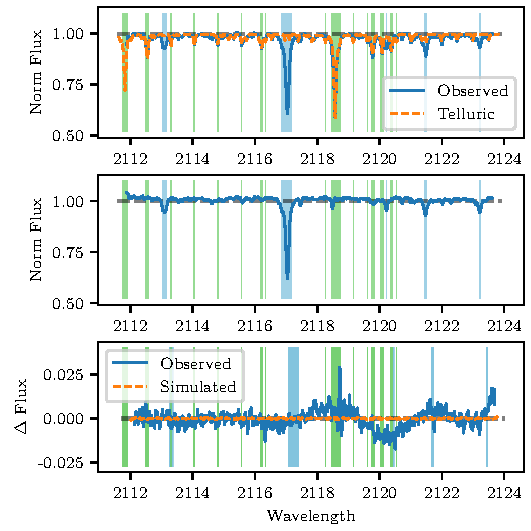
\includegraphics[width=0.8\hsize]{figures/direct-recovery/differential.pdf}\\
    \caption[Example of the spectral differential technique.]{Top: A reduced {CRIRES} observation of {HD\,30501} (blue) for detector 1 between 2112--2124\nm{} along with the {TAPAS} telluric absorption model ({orange} dashed) used for the wavelength calibration and telluric correction.
        Middle: The telluric corrected spectra.
        Bottom: ({blue}) Differential spectra for {HD\,30501} between observations 1 and 3.
        ({orange} dashed) Simulated ``perfect'' differential using {PHOENIX-ACES} spectra with parameters \Teff{}=2500\K{}, \Logg{}=5.0, and \feh{}=0.0, with the same \(\Delta {RV}\) as the observations.
        The shaded regions indicate where the telluric {green} and host star {blue} spectra are \(> 4\%\) deep.}
    \label{fig:spectral_example}
\end{figure}

The spectral differential procedure outlined above was applied to the wavelength-calibrated, telluric- and barycentre-corrected {CRIRES} observations.
The spectra were first Doppler shifted to the rest frame velocity of the system by applying a shift of \(-\gamma\).
Each spectra is then shifted by its $-{RV}_{1}$ so that the host lines are at rest.
Finally one spectrum is subtracted from the other as described above.

Although this is attempted on all targets, only the most favourable case, {HD\,30501}, is shown in \cref{fig:spectral_example}.
It is favourable because it is the second largest companion in the sample at 90~\Mjup{} but also has the second largest {RV} separation between observations.
The top panel shows the reduced CRIRES spectrum of {HD 30501} from detector 1 without telluric correction.
The telluric model is also shown in the top panel.
The middle panel shows the CRIRES spectra corrected with the telluric model.
The differential spectra recovered for {HD\,30501} is shown at the bottom panel of \cref{fig:spectral_example}.
The shaded regions indicate where the telluric {green} and host star {blue} spectra are \(> 4\%\) deep.
This indicates that the features of the differential spectrum near these shaded regions are likely due to imperfect telluric correction and host cancellation.

The mutual cancellation of the stellar host seems to work well for the \(\sim\)40\% deep line near 2117\nm{}, with the line being completely removed, but it does not do so well for the smaller \(\sim\)10\% deep line around 2121.5\nm{}.
The residual for the large \(\sim\)40\% deep telluric line near 2118.5\nm{} is still quite prominent.
Around 2120\nm{} there is wide negative residual around three neighbouring telluric lines, \(\sim\)10\% deep.
One possible explanation for this is that the continuum normalization near 2120\nm{} was influenced by this grouping of lines.

To understand the observed differential signal, a series of simulations were performed of a differential spectrum of {HD\,30501} using a synthetic {PHOENIX-ACES} spectra with parameters \Teff{}=2500\K{}, \Logg{}=5.0, and \feh{}=0.0, with the {RV} offset estimated from the observation times.
These parameters represent an estimated companion \Teff{} with the metallicity and \Logg{} similar to the host (closest grid model).
The model spectra were convolved to \(\R=50\,000\), continuum normalized and scaled by the estimated flux ratio of the companion.
In this simulation a synthetic host or telluric spectra is not included and as such simulates the differential result of a ``perfect'' host cancellation with no telluric contamination present.
This is the ideal-case scenario, and it is stressed that it is impossible to simulate the effect of improper telluric correction in a meaningful way.
When comparing the simulated and observed differential in the bottom panel of \cref{fig:spectral_example}, there is a striking amplitude difference.
The orange-dashed line of the simulated differential spectrum amplitude is of a much smaller scale than the observed differential.
This simulation demonstrates that the expected amplitude of the differential signal of {HD 30501} is much smaller than the residuals created by the differential technique applied to these observations.

The amplitude of the differential signal is lower than expected due to the very low \(\Delta {RV}\) between the observation pairs.
The maximum \(\Delta {RV}\) between observational pairs, for the targets investigated in this work, are provided in \cref{tab:estimated_rv}.
In the best target in this sample, {HD\,30501}, the \(\Delta {RV}_2\) of the companion between observations is 1.41\kmps{}.
For comparison, a single Gaussian absorption line, to be shifted by \(\Delta\lambda = {\fwhm}\) would need a \(\Delta {RV}\) of \(v_{\fwhm} = c/\R \approxeq\sim6\)\kmps{}.
Since the \(\Delta {RV}_2\) are shifted by a significant smaller value than the line {\fwhm}, the spectral lines of the companion also mutually cancel themselves, diminishing the amplitude of the differential signal significantly.
As the companion spectra are already faint (with a flux ratio at the percent level) the differential signal is not detectable in these observations at the achieved noise level.

When the \(\Delta {RV}\) of the companion is smaller than the {\fwhm} of a line, if the mutual subtraction of the host is performed, there is also a mutual subtraction of the companion spectra, diminishing the detected amplitude of the differential signal and reducing the ability to detect the companions using this method.
The observations need to be spaced further apart in time/phase to achieve a larger \(\Delta {RV}_2\) separation and increase the amplitude of the differential.
Once there is a separation there will be complex interactions between neighbouring lines that need to be accounted for.




%!TEX root = ../../thesis.tex


\subsection{Relative differential amplitude}
\label{subsec:relative_differential_amplitue}
Further investigation was performed into the differential subtraction under small \(\Delta {RV}\).
This is done by exploring the amplitude of the differential against a variation in {RV}.
Simulations were performed creating a differential spectra for a range of \(\Delta {RV}\)s between \(\pm10\)\kmps{} using the same {PHOENIX-ACES} spectra for the companion of {HD\,30501} (\Teff{}=2500\K{}, \Logg{}=5.0, \feh{}=0.0) convolved to \(\R=50\,000\).
These simulations were focus on the wavelength range 2110--2123\nm{}, corresponding to detector \#1 of the {CRIRES} observations.
The differential spectra was created for each by taking the synthetic spectrum for the companion, Doppler shifting a copy of the spectrum and subtracting it from the original.
At each {RV} step the maximum absolute differential amplitude (peak to peak) of the simulated differential spectrum observed was recorded.
Again these simulations are performed assuming perfect telluric correction and removal of the host star by only considering the spectrum of the companion alone.

The result of this simulation is shown in \cref{fig:diff_amp}.
As this absolute amplitude is specific to the lines present in the analysed wavelength range, the values were normalized by the median amplitude value outside of the line {\fwhm} (dashed vertical lines), between \(\pm(7-10)\)\kmps{}, to give a relative differential amplitude, independent from the depth of a specific line.
Differential subtraction simulations were also performed using a spectrum made up of a single Gaussian or Lorentzian line; these are shown in \cref{fig:diff_amp} as the orange dashed and green dash-dotted lines respectively.
The spectral profile shape of the differential for the Gaussian line was also checked for consistency with the analytical form of the differential spectra from~\citet[][Equation~A.1]{ferluga_separating_1997} (included above as \cref{eqn:sprofile_gaussain}).

\cref{fig:diff_amp} shows that with a \(\Delta {RV}\) of zero between companion spectra the spectral lines of the companion completely cancel each other out, resulting in zero amplitude.
As the {RV} separation increases in either direction, the individual lines stop completely cancelling begin as they begin to separate.
A maximum differential amplitude is achieved when the individual lines are fully separated.
The shape/width of the differential spectral lobes~\citet[e.g.][eqn.~A.1]{ferluga_separating_1997} was not considered, but this could also have been measured.

At simulated separations beyond 10\kmps{} the neighbouring spectral lines begin to strongly interfere, leading to a variable (quasi-sinusoidal) relative amplitude, although this is not shown here.
The shape of the relative amplitude becomes complicated due to the line interaction and because the \(\Delta {RV}\) for all observations fall well short of this region it was not investigated further.
It is suspected that the interaction of neighbouring lines is one possible cause for the difference in the relative differential amplitude between the single theoretical line profiles and synthetic spectrum between 2 and 6\kmps{}.

The vertical dotted lines indicate the line \(\rm {\fwhm} = \lambda /\R=v /c\) with a velocity of 6\kmps{} at 2\um{} with \R=50\,000, showing that the amplitude is almost maximum when the lines are separated beyond their line width.
The two solid vertical lines in \cref{fig:diff_amp} indicate the \(\Delta \textrm{RV}\)=1.41\kmps{} separation calculated for our best target, {HD\,30501} from \cref{tab:estimated_rv}, given known orbital parameters and the observation times.
This shows that our differentials have severely reduced amplitude, \(<20\%\) relative to well separated individual lines.
As the companion spectra are already faint and in combination with a host star at >1\% flux ratio the >80\% extra reduction in signal amplitude makes this detection impossible with these observations.

\begin{figure}
    \centering
    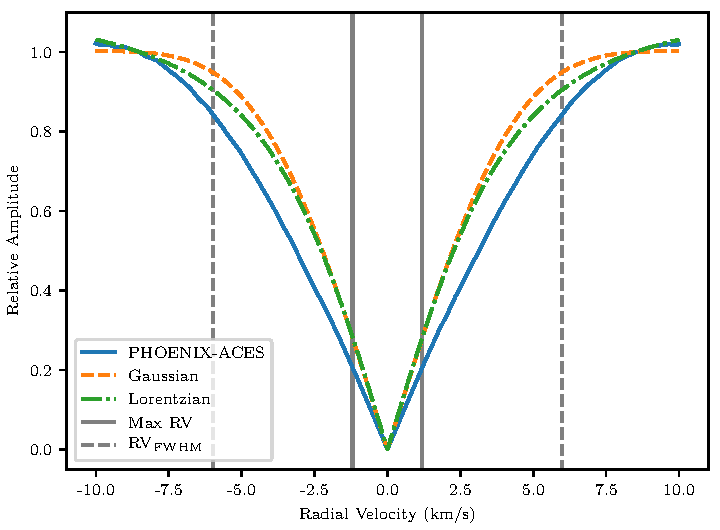
\includegraphics[width=0.8\textwidth]{figures/direct-recovery/rv_diff_final.pdf}
    \caption[Simulated relative amplitude of differntial spectrum.]{Simulated relative amplitude of differential spectra at different companion \(\Delta {RV}\) separations revealing the diminished amplitude at very small orbital separations.
        The solid blue line shows the maximum relative amplitude of the differential signal (from a shifted copy of itself) of a {PHOENIX-ACES} spectrum with \Teff{}=2500\K{}, \Logg{}=5.0, \feh{}=0.0 in the wavelength region 2110--2123\nm{}.
        The maximum difference is normalized by the median amplitude between \(\pm7\)--10\kmps{}, representing a complete line separation.
        The orange (dashed) and green (dot-dashed) lines represent the relative amplitude of a spectrum differential for a spectrum containing a single Gaussian or Lorentzian absorption line respectively, each with a unitary amplitude and a \(\rm {\fwhm} = \lambda / R\).
        The solid vertical lines indicate the estimated companion \(\Delta {RV}\) in these observations while the dashed vertical lines indicate the {RV} corresponding to the {\fwhm} at this wavelength and resolution.}
    \label{fig:diff_amp}
\end{figure}



%!TEX root = ../../thesis.tex

\section{Orbital Solutions}
\label{sec:orbtial_diagrams}
The insufficient observational spacing becomes clear when the orbits are visualized by plotting the {RV} variation.
\Crefrange{fig:hd4747p89}{fig:hd30501p89} show the {RV} curves for each target observed for this project.
The target stars that have two companions are shown twice, with each companion treated as a single Keplerian (ignoring the presence of the other companion).
For each figure the left hand plot shows the {RV} variation across a full orbit of the companion, while the plot on the right shows the {RV} variation for the 6 month observation window of {Period 89} only.
The solid black line indicates the {RV} of the host star (with scale on the left hand axis), while the blue dashed line shows the {RV} of the companion (with the scale on the right hand axis).
The orange crosses and red stars indicate on the {RV} curves the times at which observations were obtained for each target, for the host and companion respectively.

The first thing that is apparent is the variation of shape of the {RV} curves.
This is normal with the variations in shape arising from the different orbital parameters of each target (provided in \cref{tab:orbitparams}).
In the left hand plots, in which a full orbit is shown, the different shapes are created from the eccentricity, \(e\), and argument of periapsis, \(\omega\).
In the right hand panels, for which a fixed time period is shown, the orbital period of the companion also plays a role.
Specifically the ratio of orbital period to the 6 month observing period determines what fraction (or multiples) of the orbit is displayed.

The {RV} curves of the star and the planet mirror each other about the systems mean velocity, \(\gamma\), with the amplitude scaled by their mass ratio, \(q\) (see \cref{eqn:q_ratio_K2}), and \(\omega\) offset by \(180^\circ\).

All the plots, apart from {HD\,4747}, have more than one observations shown, although it can be difficult to see as the observational spacing is small.

For the companions {HD\,162020}b (\cref{fig:hd162020p89}) and {HD\,168443}b (\cref{fig:hd168443bp89}) their orbital periods are shorter than 6 months, allowing for multiple orbits to occur during {Period 89}.
As such the full amplitude range was available to measure in the observing period if observations were taken at correct times, at the locations of the extrema.
It should have been possible to obtain observations in which the companion spectra were sufficiently separated for the differential separation technique.
However in reality, the two observations for these two targets were taken immediately after each other, making any differential extremely small.
This is ignoring the fact that the flux ratios (from \cref{tab:estimated_flux_ratios}) for these short period companions are estimated to be very low, meaning they would have been very difficult to detect even if observed at the extrema.

The larger companion {HD\,168443}c in \cref{fig:hd168443cp89} has a longer orbital period, so it appears as a straight line in the right hand panel, although the amplitude variation of the companion during {Period 89} is about 8--9\kmps.
Therefore observations taken at the extreme ends of {Period 89} may have provided just enough separation to be suitable for the differential.

For HD\,202206 about 3/4 of the orbit is covered in {Period 89} with a {RV} amplitude of the companion possible of over 40\kmps{}.
Therefore, in this case well separated {RV}s could have been obtained.

For the remaining targets with long periods, it is clear that sufficiently separated {RV}s were not obtained, but also that they were not possible within a single observing period with a {RV} variation less than 6\kmps{} during {Period 89}.
For HD\,30501 the largest time separation between observations obtained is clearly visible in \cref{fig:hd30501p89}.
Unfortunately, this did not result in a large enough companion separation.
Looking at the full period, if the observations had been obtained in the previous period then sufficient separation could have possibly been obtained.

The code used to create orbital plots similar to those shown here is available under the \href{https://github.com/iastro-pt/ObservationTools}{iastro-pt/Observationtools} \emph{Github} repository with documentation available on \href{https://ia-observationtools.readthedocs.io/en/latest/rv.html}{Read the Docs}.

The sampling of points in the orbit reveal that the choice of points was not favourable for the application of the direct subtraction technique.
This was unfortunately discovered after attempting to apply the technique.

%!TEX root = ../thesis.tex
% Plotting the orbital plots for each target

\begin{figure}
    \centering
    \begin{tabular}{cc}
        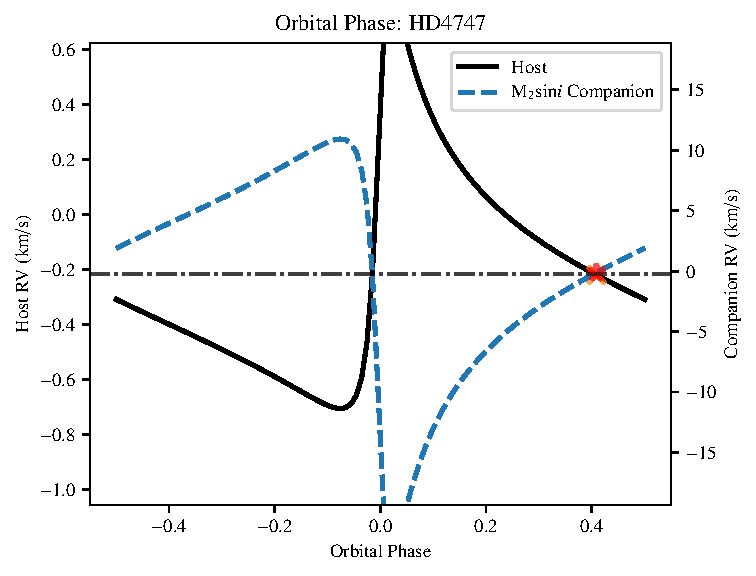
\includegraphics[width=0.45\linewidth]{figures/direct-recovery/orbital-plots/HD4747_orbital_phase.pdf} & 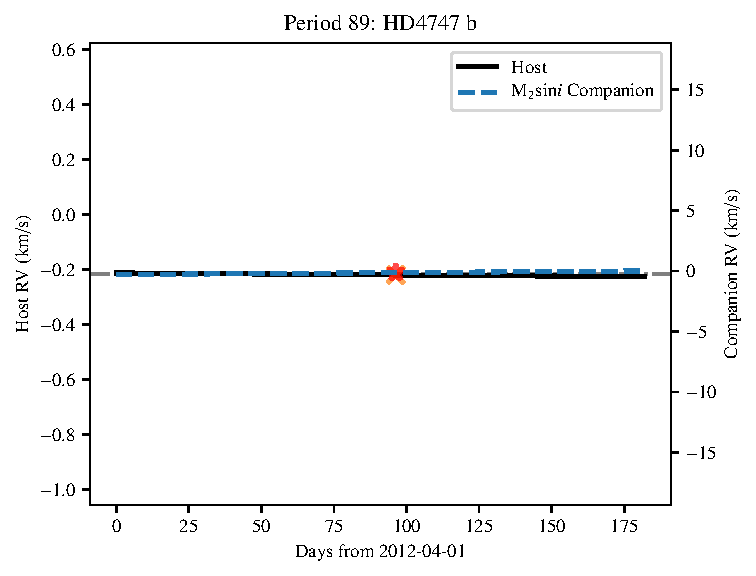
\includegraphics[width=0.45\linewidth]{figures/direct-recovery/orbital-plots/HD4747_p89.pdf}\\
    \end{tabular}
    \caption[]{{RV} single companion Keplerian orbit for {HD\,4747}.
        The left hand plot shows the {RV} curve for one full orbit while the right hand panel shows the {RV} curve over 6 months (Period 89).
        The solid black line indicates the {RV} of the host star (with scale on the left), while the blue dashed line indicates the {RV} of the companion (with scale on the right axis).
        The orange crosses and red stars indicate the times at which observations were obtained for the target, for the host and companion respectively.}
    \label{fig:hd4747p89}
\end{figure}

\begin{figure}
    \centering
    \begin{tabular}{cc}
        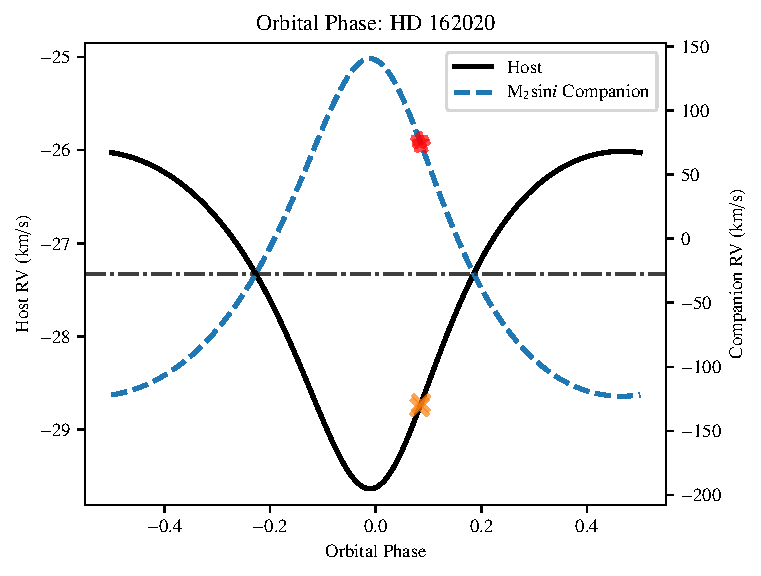
\includegraphics[width=0.45\linewidth]{figures/direct-recovery/orbital-plots/HD162020_orbital_phase.pdf} &
        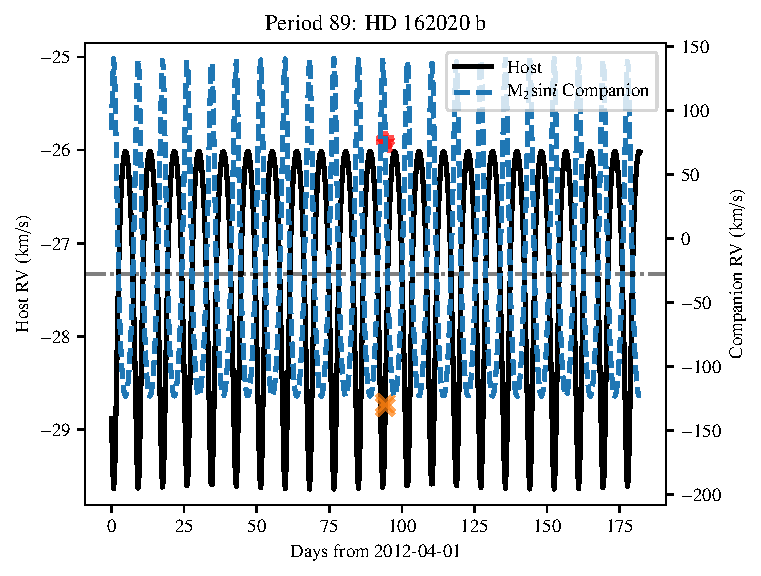
\includegraphics[width=0.45\linewidth]{figures/direct-recovery/orbital-plots/HD162020_p89.pdf}\\
    \end{tabular}
    \caption[]{Same as \cref{fig:hd4747p89} but for {HD\,162020}.}
    \label{fig:hd162020p89}
\end{figure}

\begin{figure}
    \centering
    \begin{tabular}{cc}
        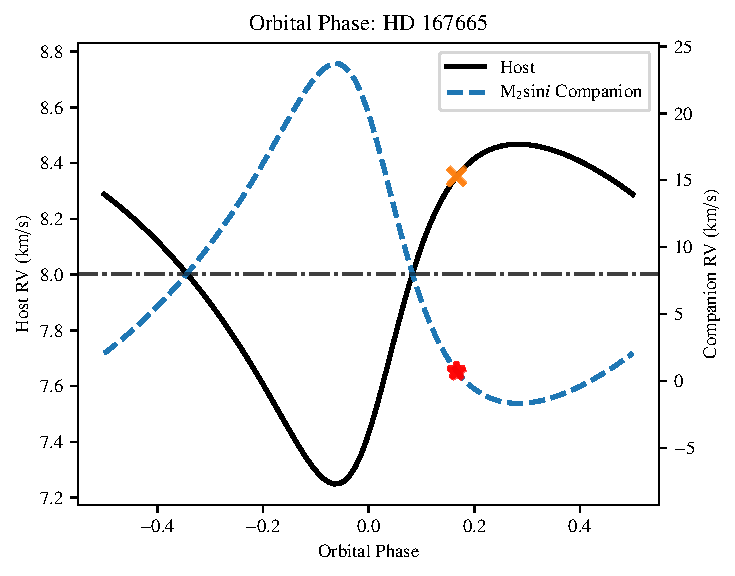
\includegraphics[width=0.45\linewidth]{figures/direct-recovery/orbital-plots/HD167665_orbital_phase.pdf} &
        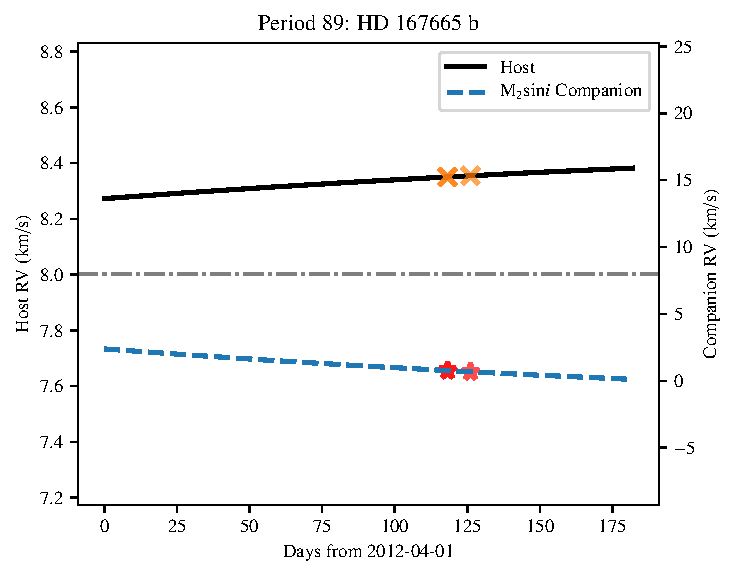
\includegraphics[width=0.45\linewidth]{figures/direct-recovery/orbital-plots/HD167665_p89.pdf}\\
    \end{tabular}
    \caption[]{Same as \cref{fig:hd4747p89} but for {HD\,167665}.}
    \label{fig:hd167665p89}
\end{figure}

\begin{figure}
    \centering
    \begin{tabular}{cc}
        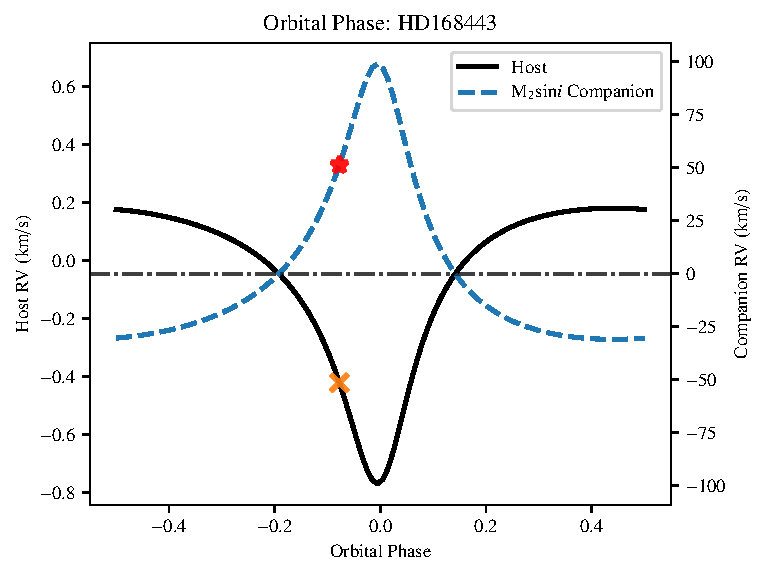
\includegraphics[width=0.45\linewidth]{figures/direct-recovery/orbital-plots/HD168443b_orbital_phase.pdf} &
        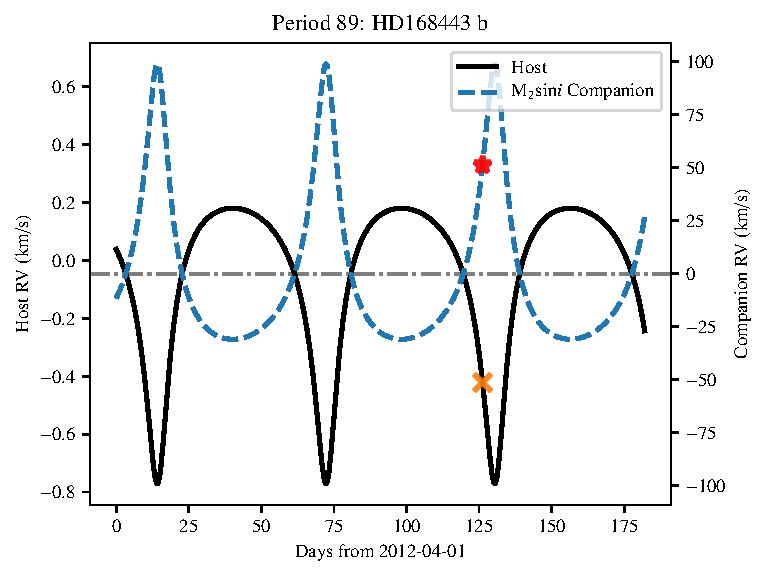
\includegraphics[width=0.45\linewidth]{figures/direct-recovery/orbital-plots/HD168443b_p89.pdf}\\
    \end{tabular}
    \caption[]{Same as \cref{fig:hd4747p89} but for {HD\,168443}b.
        Analysed as if this was a single companion.}
    \label{fig:hd168443bp89}
\end{figure}

\begin{figure}
    \centering
    \begin{tabular}{cc}
        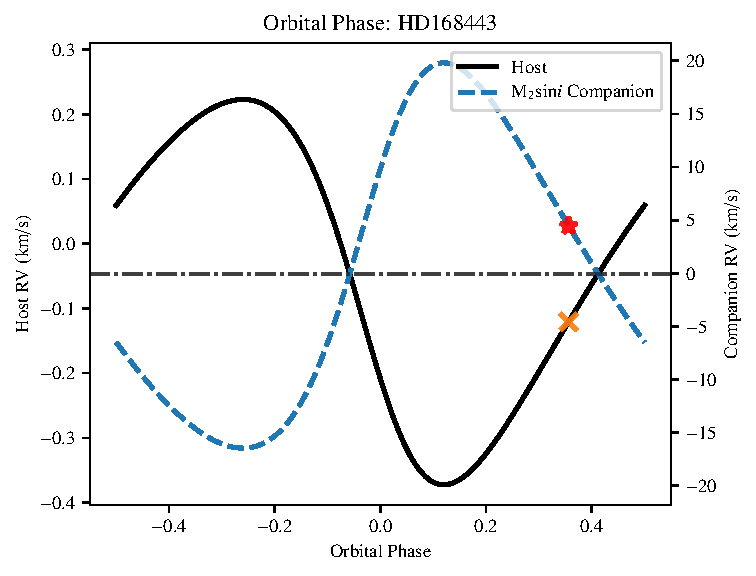
\includegraphics[width=0.45\linewidth]{figures/direct-recovery/orbital-plots/HD168443c_orbital_phase.pdf} &
        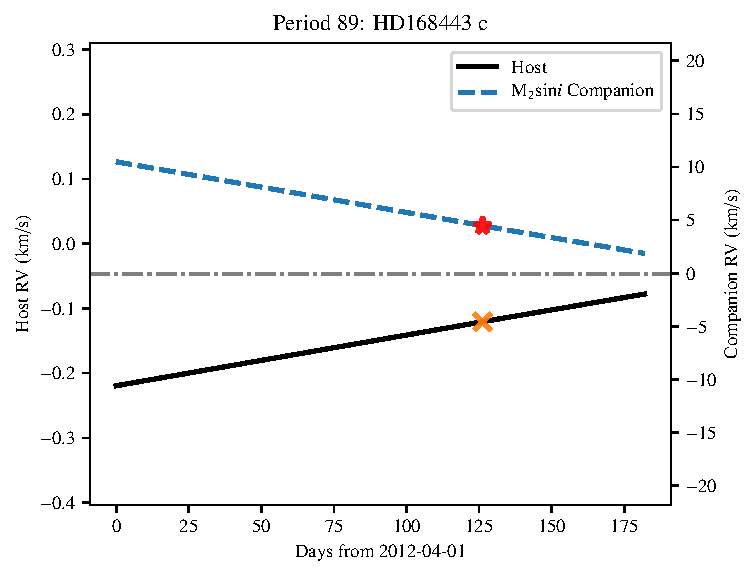
\includegraphics[width=0.45\linewidth]{figures/direct-recovery/orbital-plots/HD168443c_p89.pdf}\\
    \end{tabular}
    \caption[]{Same as \cref{fig:hd4747p89} but for {HD\,168443}c.
        Analysed as if this was a single companion.}
    \label{fig:hd168443cp89}
\end{figure}

\begin{figure}
    \centering
    \begin{tabular}{cc}
        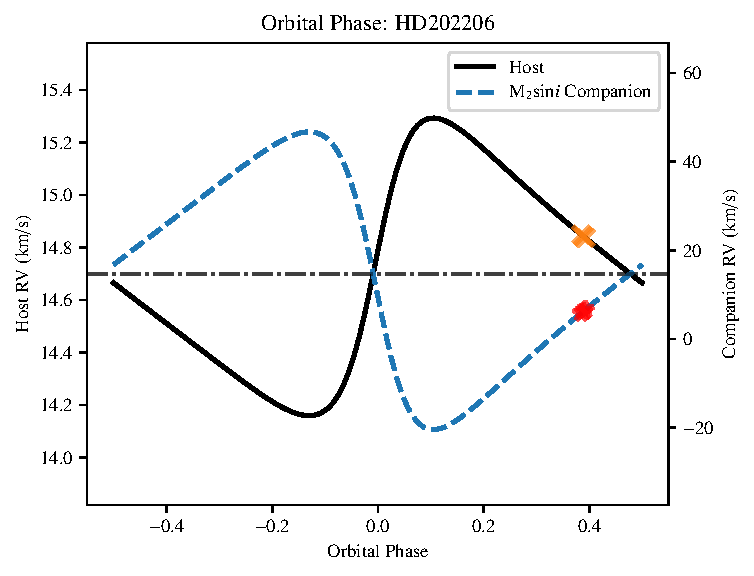
\includegraphics[width=0.45\linewidth]{figures/direct-recovery/orbital-plots/HD202206B_orbital_phase.pdf} &
        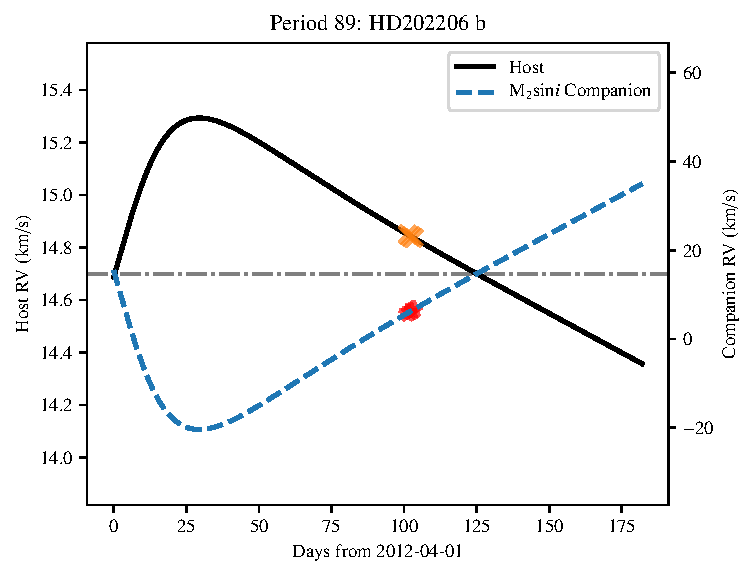
\includegraphics[width=0.45\linewidth]{figures/direct-recovery/orbital-plots/HD202206B_p89.pdf}\\
    \end{tabular}
    \caption[]{Same as \cref{fig:hd4747p89} but for {HD\,202206}B.
        Analysed as if this was a single companion.}
    \label{fig:hd202206bp89}
\end{figure}

\begin{figure}
    \centering
    \begin{tabular}{cc}
        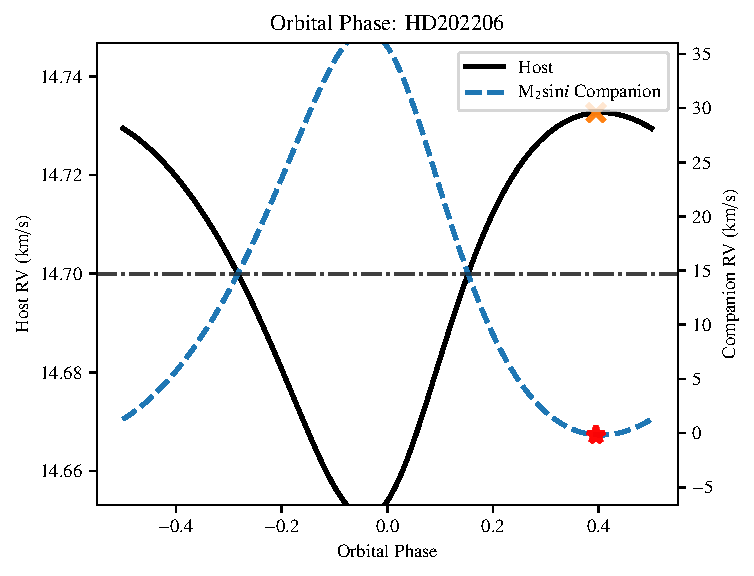
\includegraphics[width=0.45\linewidth]{figures/direct-recovery/orbital-plots/HD202206c_orbital_phase.pdf} &
        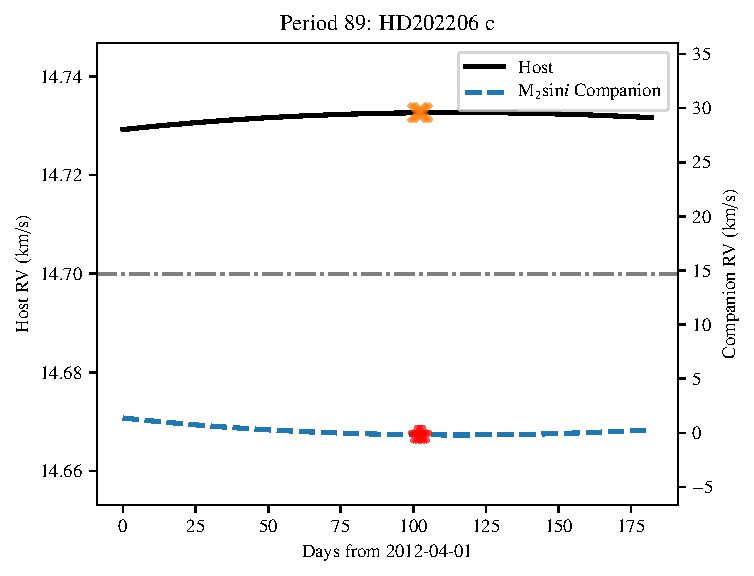
\includegraphics[width=0.45\linewidth]{figures/direct-recovery/orbital-plots/HD202206c_p89.pdf}\\
    \end{tabular}
    \caption[]{Same as \cref{fig:hd4747p89} but for {HD\,202206}c.
        Analysed as if this was a single companion.}
    \label{fig:hd202206cp89}
\end{figure}

\begin{figure}
    \centering
    \begin{tabular}{cc}
        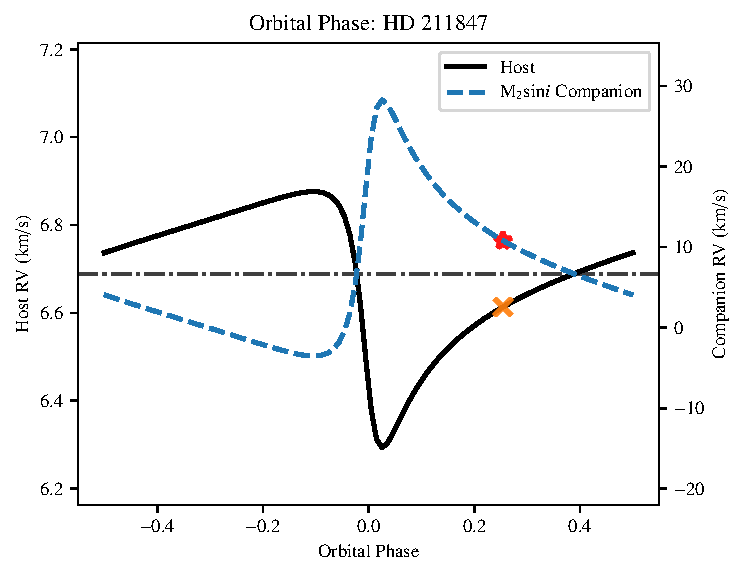
\includegraphics[width=0.45\linewidth]{figures/direct-recovery/orbital-plots/HD211847_orbital_phase.pdf} &
        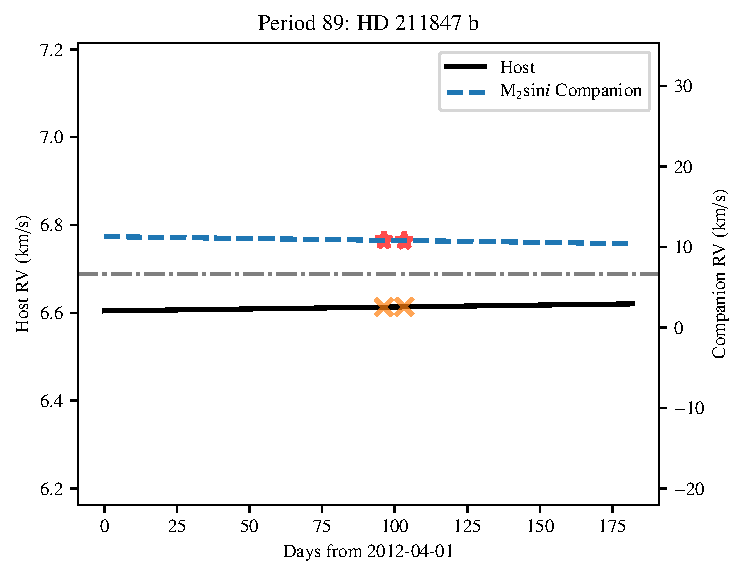
\includegraphics[width=0.45\linewidth]{figures/direct-recovery/orbital-plots/HD211847_p89.pdf}\\
    \end{tabular}
    \caption[]{Same as \cref{fig:hd4747p89} but for {HD\,211847}.}
    \label{fig:hd211847p89}
\end{figure}

\begin{figure}
    \centering
    \begin{tabular}{cc}
        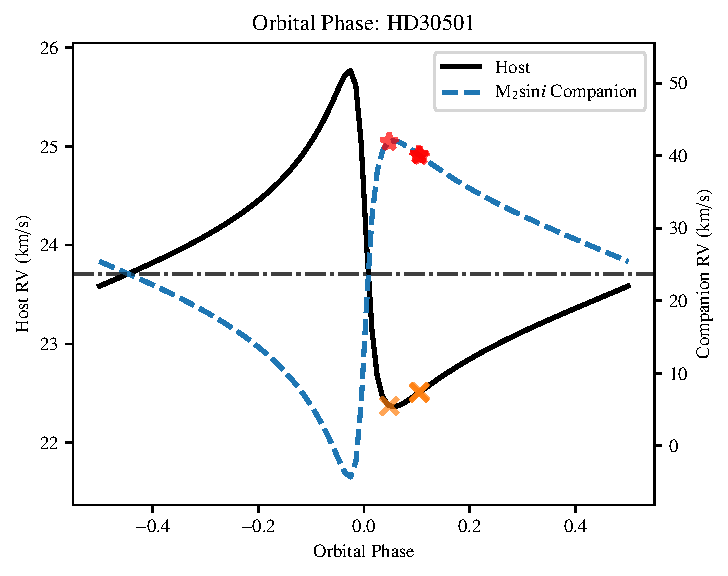
\includegraphics[width=0.45\linewidth]{figures/direct-recovery/orbital-plots/HD30501_orbital_phase.pdf} &
        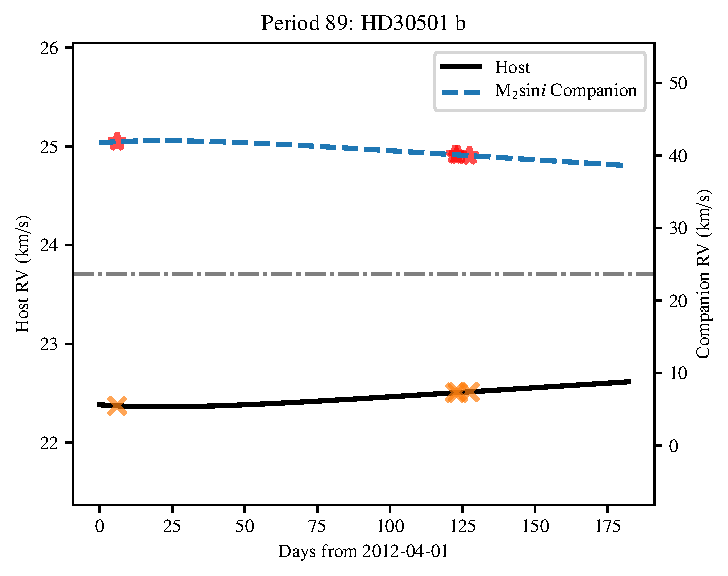
\includegraphics[width=0.45\linewidth]{figures/direct-recovery/orbital-plots/HD30501_p89.pdf}\\
    \end{tabular}
    \caption[]{Same as \cref{fig:hd4747p89} but for {HD\,30501}.}
    \label{fig:hd30501p89}
\end{figure}

% Add to list of figures.
\addtocontents{lof}{\protect\contentsline{figure}{\ref{fig:hd4747p89}--\ref{fig:hd30501p89} \quad {\color{hrefurlcolor} {RV} curves for the host and companion of each target.}}{{\color{black}\pageref{fig:hd4747p89}}}{}}




%!TEX root = ../../thesis.tex

\subsubsection{Differential scheduling challenges}
\label{subsubsec:differential-schedualing}
This work has revealed that care needs to be taken in planning the observations for the application of the spectral differential technique of faint companions in the future.
Future attempts need to pay attention in particular to: the {\fwhm} of the lines in the region (governed by resolution and wavelength), the estimated companion separation \(\Delta {RV}_2\); and the previous observations from different observing periods, all while keeping the detector settings consistent.

The original goal for the observations was to obtain two different and ``clearly separated radial-velocities'' for the secondary companion.
However, the program was assigned a low-priority (C, in {ESO} grading) and, possibly due to operational reasons, the original time requirements necessary to secure well separated {RV}s for the companion spectra could not be met.
This meant that all observations were insufficiently separated to extract a differential spectra for the companion.

The long orbital periods of these targets is also a strong contributing factor to the insufficient separations.
Most of the targets observed here have orbital periods much longer than an observing semester (183 days).
An optimal pair of observations (achieved at the extrema) would need to have been obtained from separate observing periods (between 2 months and 19 years apart).
In some cases, even observations taken at the beginning and end of a single observing semester would not be sufficient to achieve a companion separation (depending on the phase and orbital parameters), requiring separate observing periods to even achieve the minimum \(\Delta \rm {RV}\) larger than the line {\fwhm}.
At the time (2012) it was impossible to ask for observation time over several semesters in a regular proposal.

This study demonstrates the importance of proposals for projects that need to be extended over several semesters or years.
In the {ESO} context, this corresponds to ``Monitoring proposals''~\citep[e.g.][pg.~18]{eso_eso_2017}.
Observations of the targets explored here, with long orbital periods in particular, would benefit from the new abilities for multi-period proposals and scheduling systems which allow for tighter scheduling constraints, such as a companion {RV} separation.

For future observations in the context of the differential subtraction technique it is suggested that the best possible orbital solution of the host and companion be used to estimate the companions' {RV} curve during the observing period, with the companion \Mtwosini{} providing an {RV} upper-limit.
Radial velocity constraints are also valid for other studies such as the detection of reflected light from exoplanets~\citep[e.g.]{martins_evidence_2015}.
Knowing the instrumental wavelength and resolution, an observing constraint can be set to avoid taking observations when the companion spectra are insufficiently separated, or the \(\Delta {RV}_2\) < {\fwhm}.
This constraint can be set using the absolute and relative \emph{time-link} constraints available in {ESO}'s {Phase 2 Proposal Preparation} (P2PP) tool.
Additionally, analysing the known orbital solution beforehand to determine {RV} constraints will also help identify the best time to observe, if observations from separate periods will be required or, if an optimally separated companion differential is even feasible.
Again the {P2PP} documentation for this observational proposal could not be obtained to check if these observations had used any of these features, which were available at the time, and set any constraints.


%!TEX root = ../../thesis.tex

\section{Contrast to other works}

As stated previously the differential technique is not new being analytically formulated for binary star separation in~\citet{ferluga_separating_1997}.
This work tried to extend this to lower contrast ratios, to a hosts with smaller companions.

For lack of high-resolution CRIRES data~\citet{kostogryz_spectral_2013} explored simulations of the differential approach to a {BD} companion of a M-dwarf star, in which the contrast ratio is around 1/50 between 1/200 and were observed at the {RV} extrema.
Their favourable wavelength choice to achieve a good contrast ratio is \emph{K}-band, as done in work, however they chose the \ce{CO} line region (\(\sim2310\)\nm{}) where there is several narrow spectral lines.
One thing explored in~\citet{kostogryz_spectral_2013} that is not considered here is the effect of rotational broadening on the mass determination, finding that it should be possible to determine the mass of a slowly rotating companion, but a fast rotating companion is more difficult.

The limitations with regards to the {RV} separation between spectral components has also been observed in other works.
Similarly to the companion-companion {RV} separation focused on here, \citet{kolbl_detection_2015} find a limitation of \(\sim 10\)\kmps{} {RV} separation required between the host and the companion.
This is because if lines of the host and companion are blended, it is likely the companion spectra will be fitted, or incorporated into the hosts spectra, making it difficult to accurately detect the companions lines a similar {RV}.
The {RV} difference between the host an companion is given in the last column of \cref{tab:observations} as \Rvtwo{}.
It can be seen {HD~4747}, {HD~202206}, and {HD~218447} do not exceed this 10\kmps{} separation with the obtained observations.



%!TEX root = ../../thesis.tex

\section{Direct recovery in the \mir{}}
\label{sec:mir}
It was investigated if this differential technique could be extended into the mid-infrared {\mir{}} domain.
There were two reasons for this: to develop experience with the {\mir{}} domain where the contrast ratios are higher, and due to the lack of high-resolution \nir{} spectrographs available at the time (see \cref{subsec:new_generation}).

{VISIR} is a \mir{} spectrograph on the {VLT}, offering diffraction-limited imaging at high sensitivity in three mid-infrared (\mir) atmospheric windows: the \emph{M}-band at 5\um{}, the \emph{N}-band between 8--13\um{} and the \emph{Q}-band between 17--20\um{}, respectively.
The use of {VISIR} to detect the spectra of Brown Dwarf companions in the {\mir{}} was briefly explored.
The candidate selected as the best target to investigate was {HD\,219828} which has a hot-Neptune (\Mtwosini{}=21\Mearth)~\citep{melo_new_2007} and a recently discovered super Jupiter (\Mtwosini{}=15.1\,\Mjup) on a long period (13 yr) eccentric orbit (e=0.81)\citep{santos_extreme_2016}.

Based on the spectra of a cool brown dwarfs in the \mir{}, and the detector configuration available at the time, the best option for the observations was the low resolution mode covering the wavelength region 8--13\um{}.
This wavelength region would have encompassed the \ce{NH4} signature at 10.5\um{} and the edge of a \ce{CH4} band at 7.7\um{}, both large features in the {BD} \mir{} spectrum.

After performing flux ratio calculations between the host and companion using the~\citet{baraffe_evolutionary_2003} models (see \cref{subsec:compaion_flux_ratio}) and considering the performance of the {VISIR} instrument and the exposure time calculator it was determined that observations with {VISIR} to achieve a \snr{} of 100 were infeasible, requiring 1000's of hours of observing time to achieve the necessary signal-to-noise level to separate the companion from a blended spectra.
For a different target, {HD\,189733} it was calculated that with an exposure time of 2 hours the \snr{} of the host and companion would be 85 and 4 respectively, using the low resolution spectroscopy mode.
As such the direct separation approach was not explored further in the \mir{}.



\section{Summary}
This chapter presented the observations that were gathered having in mind the application of a differential subtraction method to recover the spectra of the faint {BD} companions.
Due to the poorly separated observation times relative to the long orbital periods, the differential subtraction method presented in \cref{sec:direct-subtraction} was revealed to be inappropriate for these observations as the {RV} separation of the companion spectra between observations is significantly smaller than the width of individual spectral lines.
The small separation of the companion causes the lines of the companion to also mutually cancel, severely reducing the residual signal to well below the available noise level.
The requirement of well separated {RV}s for the companion spectra was clearly stated in the original proposal but was not satisfied by the observations, however the very large orbital periods of some of the targets would not produce a sufficient {RV} signal during one semester was possibly an oversight during the proposal stage.
In the following chapter a different technique will be explored in the attempt to extract details of the companion from these observations.
